\section{Summary of Differences}
\label{summary_diff}
EfficientZero V2 builds upon EffcientZero algorithm \citep{ye2021mastering}. This section demonstrates the major applied changes to achieve mastering performance across domains.
\begin{itemize}
    \item \textbf{Search}: Different from the MCTS in EfficientZero, we employ Gumbel search which differs in action selections. Gumbel search guarantees policy improvement even if with limited simulation budgets, which significantly reduces the computation of EZ-V2.
    \item \textbf{Search-based Value Estimation}: Compared to the adaptive TD method used in EfficientZero's value estimation, we employ the empirical mean of the search root node as the target value. The search process utilizes the current model and policy to calculate improved policy and value estimation, which can improve the utilization of early-stage transitions.
    \item \textbf{Gaussian Policy}: Inspired by Sampled MuZero \citep{hubert2021learning}, we employ an Gaussian distribution, which is parameterized by the learnable policy function, to represent the policy in continuous action spaces. We generate search action candidates by simply sampling from the Gaussian policy, which naturally satisfies the sampling without replacement in Gumbel search. We then prove the policy improvement of Gumbel search still holds in the continuous setting.
    \item \textbf{Action Embedding}: We employ an action embedding layer to encode the real actions as latent vectors. By representing actions in a hidden space, actions that are similar to each other are placed closer in the embedding space. This proximity allows the RL agent to generalize its learning from one action to similar actions, improving its efficiency and performance.
    \item \textbf{Priority Precalculation}: Conventionally, the priorities of a newly collected trajectory are set to be the maximal priority of total collected transitions. We propose to warm up the new priorities by calculating the bellman error using the current model. This increases the probability of newly collected transitions being replayed, thereby improving sample efficiency.
    \item \textbf{Architecture}:
    For the 2-dimensional image inputs, we follow the most implementation of the architecture of EfficientZero. For the continuous control task with 1-dimensional input, we use a variation of the previous architecture in which all convolutions are replaced by fully connected layers. The details could be found in Appendix \ref{arch}.
    \item \textbf{Hyperparameters}: We tuned the hyperparameters of EfficientZero V2 to achieve satisfying performance across various domains. The generality is verified by training from scratch without further adjustments, including Atari 100k, Proprio Control, Vision Control. More details refer to Appendix \ref{hyper-param}.
\end{itemize}

% \section{Proof of Policy Improvement}
% \label{policyproof}
% Intuitively, we would like to obtain an action better than the current policy $\pi$. Therefore, if the action selected can make policy improvement, there exists:
% \begin{equation}
%     \label{app:pi}
%     \mathbb{E}\left[q\left(a^*_{S}\right)\right] \geq \mathbb{E}_{a \sim \pi}[q(a)]
% \end{equation}
% where $a^*_{S}$ represents the best action chosen from the tree search. In Gumbel Muzero, the following equation holds and the planning with Gumbel produces a policy improvement.
% \begin{equation}
%     \label{gumbelq}
%     \begin{split}
%         q(\underset{a \in \mathcal{A}_{\text {topn }}}{\arg \max }(g(a) +\operatorname{logits}(a)+ \sigma(q(a)))) \geq q(\underset{a \in \mathcal{A} \text { topn }}{\arg \max }(g(a)+\operatorname{logits}(a)))    
%     \end{split}
% \end{equation}
% In Appendix B of Gumbel Muzero, they demonstrate that it holds for the expectation: $\mathbb{E}\left[q\left(a^*_{S}\right)\right] \geq \mathbb{E}_{a \sim \pi} [q(a)]$ in discrete action space.

% Inspired by Gumbel Muzero, we can get a similar inequality like Equation \eqref{gumbelq}. Furthermore, the policy improvement holds when the sampling actions approach infinity. 
% In Equation \ref{gumbelq}, $\underset{a \in \mathcal{A} \text { topn }}{\arg \max }(g(a)+\operatorname{logits}(a))$ is equivalent to sampling from the  policy network $p$. Considering the continuous control, we can directly sample actions from the policy network. Let $\hat{p}=\frac{1}{K} \sum_i \delta_{a, a^i}$ as the corresponding empirical distribution which is non-zero only on the sampled actions $a^i$. Due to using K actions in Gumbel search, we can resemble the empirical distribution $\hat{p}$ as a discrete distribution in the previous method. 

% According to Definition \ref{def:PI}, we can rewrite it under the expectation of $\hat{p}$ as: $\sum_{a\in\mathcal{A}}\hat{p}q(a)$. According to the new definition of the Gumbel score $\sigma(\hat{q})$, the right-side of Equation \eqref{PI} can be rewritten as: $q(\underset{a \sim \hat{p}}{\arg \max}(\sigma(q(a))) )
% $. Apparently, the following formula holds because $\sigma(\cdot)$ is a monotonically increasing transformation.
% \begin{equation}
%     q(\underset{a \sim \hat{p}}{\arg \max}(\sigma(q(a))) )\geq\sum_{a\in\mathcal{A}}\hat{p}q(a)
% \end{equation}
% As $K \rightarrow \infty$, we obtain
% \begin{equation}
%     \begin{split}
%        \underset{K \rightarrow \infty}{\lim}q(\underset{a \sim \hat{p}}{\arg \max}(\sigma(q(a))) ) &\geq \underset{K \rightarrow \infty}{\lim}\sum_{a\in\mathcal{A}} \hat{p}q(a)\\
%         \mathbb{E} [q(\underset{a \sim \hat{p}}{\arg \max}(\sigma(q(a))) )] &\geq
%         \mathbb{E}_{a \sim p} q(a) \\ 
%     \end{split}
% \end{equation}
% This is because we replace the limit of a sum with the expectation. Furthermore, $\underset{a \sim \hat{p}}{\arg \max}(\sigma(q(a)))$ actually equals $a^*_S$ in a whole search. Until now, we have demonstrated that policy improvement exists in the sampling-based Gumbel search.

% \section{Gumbel-Top-k Trick}
% \label{gumbel_topk}
% The Gumbel-Top-k trick \citep{kool2019stochastic} can choose the top $n$ actions without replacement in a categorical distribution $\pi$. Specifically, the action sample $A$ can be sampled by the Gumbel-Max trick, which is defined as follows.
% \begin{equation}
% \begin{aligned}
% \left(g \in \mathbb{R}^k\right) & \sim \operatorname{Gumbel}(0) \\
% A & =\underset{a}{\arg \max }(g(a)+\operatorname{logits}(a)) 
% \end{aligned}
% \end{equation}
% where $\operatorname{logits}(a)$ is the logit of the action a, and $g$ is a vector of $k$ Gumbel variables. Hereafter, we can sample $n$ actions without replacement. 
% \begin{equation}
% \begin{aligned}
% A_1 & =\underset{a}{\arg \max }(g(a)+\operatorname{logits}(a)) \\
% \vdots & \\
% A_n & =\underset{a \notin\left\{A_1, \ldots, A_{n-1}\right\}}{\arg \max }(g(a)+\operatorname{logits}(a)) .
% \end{aligned}
% \end{equation}
% Furthermore, we denote the set of $n$ top actions by $\operatorname{argtop}(g + logits, n) = {A_1, A_2,..., A_n}$.



\section{Calculation of Target Policy}
\label{cal_ip}

In discrete control, the calculation of the target policy is the same as that of the original Gumbel search, which can be found in Gumbel Muzero \citep{danihelka2021policy}.
In a continuous setting, we modify the calculation of target policy as follows.
\begin{equation}
    \pi^{\prime}=\text{softmax}(\sigma(\text{completedQ}))
\end{equation}
where completedQ is a comprehensive value estimation of visited and unvisited candidates. For visited nodes, the completedQ is calculated via the empirical estimation as $q(a)=r(s,a)+\gamma v(s^\prime)$, $v(s^\prime)$ is the empirical mean of bootstrapped value sum and visit counts. For non-visits, $\text{completedQ}$ is estimated through the weighted average Q-value of visited nodes as $\sum_{a}\pi(a)q(a)$.  

We mention the transformation $\sigma$ is a monotonically increasing transformation in the main text. For a concrete instantiation of $\sigma$, we use
\begin{equation}
\sigma(q(s,a))=\left(c_{\text {visit }}+\max _b N(b)\right) c_{\text {scale }}q(s,a)
\end{equation}
where $\max _b N(b)$ is the visit count of the most visited action. $c_{\text {visit }}$ and $c_{\text {scale }}$ are 50 and 0.1 respectively.


\section{Advantage of Simple Policy Loss}
\label{simplepi}

Different from minimizing the cross-entropy between the policy with the target policy, the simple loss using $a^*_S$ directly improves the possibility of the recommended action in tree search. That means we can make the policy network output a good action in the early stage. With the iteration repeating, the policy network can find the optimal point. More specifically, we provide an intuitive example to illustrate that the policy can reach the optimal point more efficiently, as shown in Fig. \ref{appb:simplepi}. The whole space represents the action space. The simple loss enforces the policy to output the current best point colored red. The original cross-entropy loss considers all actions and thus makes the policy's output near the point colored brown. We can see that when the action space is large, the red point can guide the policy to reach the optimal point colored purple more quickly.

\begin{figure}[h]
\centering
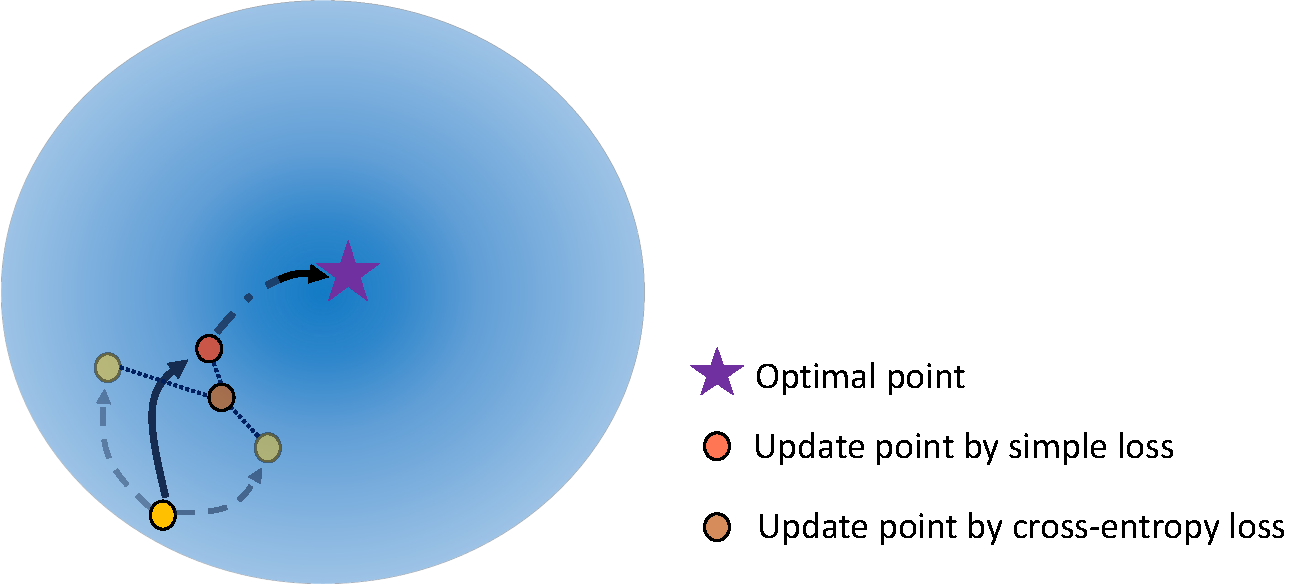
\includegraphics[width=0.5\textwidth]{sections/figs/app-1.pdf}
\caption{Intuitive example showing the difference between simple policy loss using $a^*_S$ and cross-entropy loss.}
\label{appb:simplepi}
\end{figure}



\section{Details of Search-based Value Estimation (SVE)}
\subsection{Calculation of SVE}
\label{cal_sve}
First, the search process expands a tree through $N$ simulations gradually. At each simulation, the agent dives to a leaf and expands a new child. The diving path is easily associated with an $H(n)$-step rollout, which forms an imagined H(n)-step value estimation for the root node. This estimation process will be repeated $N$ times, to get an average estimation, as defined in Definition \ref{app:def:sve}.

\begin{definition}[\textbf{Search-Based Value Estimation}]
\label{app:def:sve}
\textit{Using imagined states and rewards $\hat{s}_{t+1}, \hat{r}_t=\mathcal{G}(\hat{s}_t,\hat{a}_t)$ obtained from our learnable dynamic function, 
% the search-based value estimation of a given state $s_0$ is defined as
the value estimation of a given state $s_0$ can be derived from the empirical mean of $N$ bootstrapped estimations, which is formulated as
}
\begin{equation}
    \hat{V}_\text{S}(s_0)=\frac{\sum_{n=0}^{N}\hat{V}_n(s_0)}{N}
\end{equation}
\textit{where $N$ denotes the number of simulations, $\hat{V}_n(s_0)$ is the bootstrapped estimation of the $n$-th node expansion, which is formulated as }
\begin{equation}            \hat{V}_n(s_0)=\sum_{t=0}^{H(n)}\gamma^t\hat{r}_t+\gamma^{H(n)}\hat{V}(\hat{s}_{H(n)})
\end{equation}
\textit{where $H(n)$ denotes the search depth of the $n$-th iteration.}
\end{definition}

\section{Proof for SVE Error Bound}
\begin{corollary}[\textbf{Search-Based Value Estimation Error}]
\label{app:theorem:sve_error}
    Define $s_t,a_t,r_t$ to be the states, actions, and rewards resulting from current policy $\pi$ using true dynamics $\mathcal{G}^*$ and reward function $\mathcal{R}^*$, starting from $s_0\sim\nu$ and similarly define $\hat{s}_t, \hat{a}_t, \hat{r_t}$ using learned function $\mathcal{G}$. Let reward function $\mathcal{R}$ to be $L_r-Lipschitz$ and value function $\mathcal{V}$ as $L_V-Lipschitz$. Assume $\epsilon_s, \epsilon_r, \epsilon_v$ as upper bounds of state transition, reward, and value estimations respectively. We define the error bounds of each estimation as
    % \begin{equation}
    %     \max_{n\in[N],t\in[H(n)]}\mathbb{E}\left[\Vert\hat{s}_t-s_t\Vert^2\right]\leq\epsilon^2
    % \end{equation}
    \begin{gather}
        \max_{n\in[N],t\in[H(n)]}\mathbb{E}\left[\Vert\hat{s}_t-s_t\Vert^2\right]\leq\epsilon_s^2 \\
        \max_{n\in[N],t\in[H(n)]}\mathbb{E}\left[\Vert\mathcal{R}(s_t)-\mathcal{R}^*(s_t)\Vert^2\right]\leq\epsilon_r^2 \\
        \max_{n\in[N],t\in[H(n)]}\mathbb{E}\left[\Vert\mathcal{V}(s_t)-\mathcal{V}^*(s_t)\Vert^2\right]\leq\epsilon_v^2
    \end{gather}
    within a tree-search process. Then we have errors
    \begin{equation}
    \begin{aligned}
        \text{MSE}_\nu(\hat{V}_\text{S})\leq\frac{4}{N^2}\sum_{n=0}^N\left(\sum_{t=0}^{H(n)}\gamma^{2t}(L_r^2\epsilon_s^2+\epsilon_r^2)+\gamma^{2H(n)}(L_V^2\epsilon_s^2+\epsilon_v^2)\right)
    \end{aligned}
    \end{equation}
    % Notably, the coefficient of $\epsilon^2$ 
    % \begin{equation*}
    %     \frac{2}{N^2}\sum_{n=0}^N\left(\sum_{t=0}^{H(n)}\gamma^{2t}L_r^2+\gamma^{2H(n)}L_V^2\right)
    % \end{equation*}
    % is convergent with $H(n)$. Additionally, 
    where $N$ is the simulation number of the search process. $H(n)$ denotes the depth of the $n$-th search iteration.
    % The upper bound will converge to 0 when the dynamic function is approximately optimal $\epsilon\to 0$.
\end{corollary}


\begin{proof}
To provide detailed proof for the upper bound of the MSE of the search-based value estimation $\hat{V}_\text{S}$, we follow a structured approach inspired by Model-based Value Estimation (MVE) \citep{feinberg2018model}, with adjustments for the specifics of MCTS and considerations of errors of reward and value estimations.

Given Definition \ref{def:sve}, we aim to bound the MSE of this estimator, defined as:
\begin{equation}
    \text{MSE}_\nu(\hat{V}_\text{S})=\mathbb{E}\left[\left(\hat{V}_\text{S}(s_0)-V_\pi(s_0)\right)^2\right]
\end{equation}
Where $V_\pi(s_0)=\sum_{t=0}^{H-1}\gamma^{t}r_t+\gamma^{H}V_\pi(s_H)$. We can first decompose the MSE as

\begin{equation}
\begin{split}
\label{e1}
    \text{MSE}_\nu(\hat{V}_\text{S})=\mathbb{E}\Bigg[ \Bigg(\frac{1}{N} \sum_{n=0}^N\Bigg(\sum_{t=0}^{H(n)}\gamma^t(\hat{r}_t-r_t) +
    \gamma^{H(n)}\left(\hat{V}(\hat{s}_{H(n)})-V_\pi(s_{H(n)})\right)\Bigg)\Bigg)^2 \Bigg]
\end{split}
\end{equation}

According to $L-Lipschitz$ continuity of $\mathcal{R}$ and Cauchy inequality, we can derive
\begin{equation*}
\begin{aligned}
    \mathbb{E}\left[(\hat{r}_t-r_t)^2\right]&=\mathbb{E}\left[(\mathcal{R}(\hat{s}_t)-\mathcal{R}^*(s_t))^2\right]\\
    &=\mathbb{E}\left[(\mathcal{R}(\hat{s}_t)-\mathcal{R}(s_t)+\mathcal{R}(s_t)-\mathcal{R}^*(s_t))^2\right]\\
    &\leq 2\mathbb{E}\left[(\mathcal{R}(\hat{s}_t)-\mathcal{R}(s_t))^2\right]+2\mathbb{E}\left[(\mathcal{R}(s_t)-\mathcal{R}^*(s_t))^2\right] (\text{Cauchy inequality})\\
    &\leq 2L_r^2\mathbb{E}\left[\Vert\hat{s}_t-s_t\Vert^2\right]+2\mathbb{E}\left[\Vert\mathcal{R}(s_t)-\mathcal{R}^*(s_t)\Vert^2\right]\\
    &\leq 2L_r^2\epsilon_s^2+2\epsilon_r^2
\end{aligned}
\end{equation*}
% \begin{equation*}
% \begin{aligned}
%     \mathbb{E}\left[(\hat{r}_t-r_t)^2\right]&\leq L_r^2\mathbb{E}\left[\Vert\hat{s}_t-s_t\Vert^2\right]\\
%     % \mathbb{E}\left[\left(\hat{V}(\hat{s}_{H(n)})-V_\pi(s_{H(n)})\right)^2\right]&\leq L_V^2\mathbb{E}\left[\Vert\hat{s}_{H(n)}-s_{H(n)}\Vert^2\right]
%     \mathbb{E}\left[\left(\hat{V}(\hat{s}_{t})-V_\pi(s_{t})\right)^2\right]&\leq L_V^2\mathbb{E}\left[\Vert\hat{s}_{t}-s_{t}\Vert^2\right]
% \end{aligned}
% \end{equation*}
Similarly, we derive the error bound of value estimation as
\begin{equation*}
    \mathbb{E}\left[\left(\hat{V}(\hat{s}_{t})-V_\pi(s_{t})\right)^2\right]=\mathbb{E}\left[(\mathcal{V}(\hat{s}_t)-\mathcal{V}^*(s_t))^2\right]\leq 2L_v^2\epsilon_s^2+2\epsilon_v^2
\end{equation*}

Assume the model inference errors are additive per step, hence
% at each step are \textit{iid}, then the total error over $h$ steps could be though of a random walk, hence
% \begin{equation*}
% \begin{aligned}
%     \mathbb{E}\left[(\hat{r}_{t+h}-r_{t+h})^2\right]&\leq  L_r^2\mathbb{E}\left[\Vert\hat{s}_{t+h}-s_{t+h}\Vert^2\right]\\
%     \mathbb{E}\left[\left(\hat{V}(\hat{s}_{t+h})-V_\pi(s_{t+h})\right)^2\right]&\leq  L_V^2\mathbb{E}\left[\Vert\hat{s}_{t+h}-s_{t+h}\Vert^2\right]
% \end{aligned}
% \end{equation*}

% Using Cauchy-Schewartz inequality $(a+b)^2\leq2a^2+2b^2$, we have
\begin{equation}
\begin{split}
    \text{MSE}_\nu(\hat{V}_\text{S})\leq& \frac{2}{N^2}\sum_{n=0}^N\Bigg(\sum_{t=0}^{H(n)}\gamma^{2t}(\hat{r}_t-r_t)^2+
    \gamma^{2H(n)}\left(\hat{V}(\hat{s}_{H(n)})-V_\pi(s_{H(n)})\right)^2\Bigg)\\
\leq&
% \frac{2\epsilon^2}{N^2}\sum_{n=0}^N\left(\sum_{t=0}^{H(n)}\gamma^{2t}L_r^2+\gamma^{2H(n)}L_V^2\right)
\frac{4}{N^2}\sum_{n=0}^N\left(\sum_{t=0}^{H(n)}\gamma^{2t}(L_r^2\epsilon_s^2+\epsilon_r^2)+\gamma^{2H(n)}(L_V^2\epsilon_s^2+\epsilon_v^2)\right)
\end{split}
\end{equation}
Considering the convergence
% whether the coefficient part 
% \begin{equation}
%     \frac{2}{N^2}\sum_{n=0}^N\left(\sum_{t=0}^{H(n)}\gamma^{2t}L_r^2+\gamma^{2H(n)}L_V^2\right)
% \end{equation}
% converges 
with increasing search depth $H(n)$, we separate it into two parts:
\begin{enumerate}
    \item \textbf{The reward error term} $\sum_{t=0}^{H(n)}\gamma^{2t}(L_r^2\epsilon_s^2+\epsilon_r^2)$:
    Given $L_r\in \mathcal{C}$, $\gamma\in(0,1)$, and $\epsilon_s,\epsilon_r$ decaying with training, the series is obviously convergent.
    % let $M(H)=\sum_{t=0}^H t\gamma^{2t}$, we have
    % \begin{equation*}
    %     M(H)-M(H-1)=H\gamma^{2H}
    % \end{equation*}
    % We need to prove $\lim_{H\to\infty}H\gamma^{2H}=0$. Using ratio method, we have
    % \begin{equation*}
    % \begin{aligned}
    %     \frac{(H+1)\gamma^{2(H+1)}}{H\gamma^{2H}}=(1+\frac{1}{H})\gamma^2<1
    % \end{aligned}
    % \end{equation*}
    \item \textbf{The terminal state value error term} $\gamma^{2H(n)}(L_V^2\epsilon_s^2+\epsilon_v^2)$ is similarly converged. 
    % to 0 if $H(n)\to\infty$.
\end{enumerate}
On the other hand, this upper bound will also converge to 0 if the model is optimal $\epsilon_s,\epsilon_r,\epsilon_v\to0$.
\end{proof}

Compared to SVE, the estimation error of multi-step TD methods in \citep{de2018multi} depends on sampling, making it difficult to determine their theoretical upper bound of estimation errors. In other words, the estimation error of multi-step TD methods increases gradually during learning due to the off-policy issue.


\section{Details of Mixed Value Target}
\label{mixedV}
The mixed value target is calculated for each transition sampled from the buffer. It contains two types of value targets: the search-based value target and the multi-step TD target.

Specifically, we use two criteria to determine if we should use a search-based value target. The first criterion is whether the sampled transition comes from recent rollouts. If the transition is not from recent rollouts, meaning the transition is considered stale, we opt for the search-based value as the target. Otherwise, the multi-step TD (Temporal Difference) target is employed. The second criterion considers whether the current training step is in the early stage. During this phase, all transitions in the buffer are fresh. Additionally, the error in the dynamic model is still significant, resulting in inaccuracies in search-based value estimation. Therefore, we opt for the multi-step TD target as the target value.

\section{Details of Achitecture}
\label{arch}
For the 2-dimensional image inputs, we follow the most implementation of the architecture of EfficientZero. For the continuous control task with 1-dimensional input, we use a variation of the previous architecture in which all convolutions are replaced by fully connected layers. In the following, we describe the detailed architecture of EZ-V2 under 1-dimensional input.

The representation function $\mathcal{H}$ first processes the observation by a running mean block. The running mean block is similar to a Batch Normalization layer without learnable parameters. Then, the normalized input is processed by a linear layer, followed by a Layer Normalisation and a Tanh activation. Hereafter, we use a Pre-LN Transformer style pre-activation residual tower \citep{xiong2020layer} coupled with Layer Normalisation and Rectified Linear Unit (ReLU) activations to obtain the latent state. We used 3 blocks and the output dim is 128. Each linear layer has a hidden size of 256.

The dynamic function $\mathcal{G}$ takes the state and the action embedding as inputs. the action embedding is obtained from the action embedding layer which consists of a linear layer, a Layer Normalization, and a ReLU activation. The size of the action embedding is 64. The combination of the state and the action embedding are also processed by Pre-LN Transformer style pre-activation residual tower \citep{xiong2020layer} coupled with Layer Normalisation and ReLU activations. 

For the reward $\mathcal{R}$, value $\mathcal{V}$ and policy $\mathcal{P}$ function share the similar network structures. Taking the state as input, a linear layer followed by a Layer Normalization obtains the hidden variables. Then, we use the MLP network combined with Batch Normalization, which is similar to that of EfficientZero, to obtain the reward, value, and policy prediction. The hidden size of each layer is 256, and the activation function is ReLU. 

The reward and value predictions used the categorical representation introduced in EfficientZero. We used 51 bins for both the value and the reward predictions with the value being able to represent values between $\{-299.0, 299.0\}$. The reward can represent values between $\{-2.0, 2.0\}$. The maximum reward is 2 because the action repeat in DMControl is 2.
For policy function, the network outputs the mean and standard deviation of the Gaussian distribution. Then we use the 5 times Tanh function to restrict the range of the mean, and Softplus \citep{zheng2015improving} function to make the standard deviation over 0. In addition, the policy distribution is modeled by a squashed Gaussian distribution. A squashed Gaussian distribution belongs to a modification of a standard Gaussian, where the outputs are transformed into a bounded interval. 

Furthermore, we add a running mean block for observation in the representation function $\mathcal{H}$ in continuous control whose observation is 1 dimension. A key benefit of the module is that it normalizes the observation to mitigate exploding gradients. 


\section{Training pipeline}
\label{pipeline}


The training pipeline comprises data workers, batch workers, and a learner. The data workers, also known as self-play workers, collect trajectories based on the model updated at specific intervals. The actions executed in these trajectories are determined using the sampling-based Gumbel search, as depicted in Figure \ref{framework} (B).

On the other hand, batch workers provide batch transitions sampled from the replay buffer to the learner. Similar to EfficientZero, the target policy and value in batch transitions are reanalyzed with the latest target model. This reanalysis involves revisiting past trajectories and re-executing the data using the target model, resulting in fresher search-based values and target policies obtained through model inference and Gumbel search.
The target model undergoes periodic updates at specified intervals during the training process. 

Finally, the learner trains the reward, dynamics, value, and policy functions using the reanalyzed batch. Figure \ref{framework} (A) and Equation \eqref{loss} illustrate the specific losses involved in the training process. To enhance the learning process, we have designed a parallel training framework where data workers, batch workers, and a learner all operate concurrently.


\section{Hyperparameters of Algorithms}
\label{hyper-param}

\subsection{Hyperparameters of Our Method}

We employ similar hyperparameters across all domains, as outlined in Table \ref{tab:hparams}. It's worth noting that we use different optimizers in tasks with different inputs. Specifically, due to architectural differences, we opt for the Adam optimizer in the 'Proprio Control 50-100k' task, whereas we utilize the SGD optimizer in 'Vision Control 100-200k' and 'Atari 100k'.

In the case of most baselines, we either adhere to the suggested hyperparameters provided by the authors of those baselines for each domain or fine-tune them to suit our setup when such suggestions are not available. Notably, SAC, DrQ-v2, and DreamerV3 employ a larger batch size of 512, while our method and EfficientZero achieve stable learning with a batch size of 256.


\begin{table}[h!]
\centering
\begin{tabular}{lcc}
% \begin{tabular}{
%   colspec = {| L{15em} | C{6em} | C{10em} |},
%   row{1} = {font=\bfseries},
% }
\toprule
\textbf{Name} & \textbf{Symbol} & \textbf{Value} \\
\midrule
\multicolumn{3}{l}{\textbf{General}} \\
\midrule
Replay capacity (FIFO) & --- & $10^6\!\!$ \\
Batch size & $\mathcal{B}$ & 256 \\
Discount & $\gamma$ & 0.997\\
Update-to-data (UTD)  & --- & 1 \\
Unroll steps & $l_{\text{unroll}}$ & 5 \\
TD steps & $k$ & 5 \\
Number of simulations in search & $N_{sim}$ & 32 (16 in `Atari 100k') \\
Number of sampled actions & $K$ & 16 (8 in `Atari 100k')\\
Self-play network updating interval & --- & 100 \\
Target network updating interval & --- & 400 \\
Starting steps when using SVE & $T_1$ & $4\cdot10^{4}$ \\
Threshold of buffer index when using SVE & $T_2$ & $2\cdot10^{4}$ \\
Priority exponent & $\alpha$ & 1 \\
Priority correction & $\beta$ & 1 \\
Reward loss coefficient  & $\lambda_1$ & 1.0 \\
Policy loss coefficient  & $\lambda_2$ & 1.0 \\
Value loss coefficient & $\lambda_3$ & 0.25 \\
Self-supervised consistency loss coefficient & $\lambda_4$ & 2.0 \\
Policy entropy loss coefficient  & --- & $5\cdot10^{-3}$ \\
\midrule
\multicolumn{3}{l}{\textbf{Proprio Control 50-100k }} \\
\midrule
Optimizer & --- & Adam \\
Optimizer: learning rate & --- & $3\cdot10^{-4}$ \\
Optimizer: weight decay & --- & $2\cdot10^{-5}$ \\
\midrule
\multicolumn{3}{l}{\textbf{Vision Control 100-200k \& Atari 100k}} \\
\midrule
Optimizer & --- & SGD \\
Optimizer: learning rate & --- & 0.2 \\
Optimizer: weight decay & --- & $1\cdot10^{-4}$ \\
Optimizer: momentum & --- & 0.9 \\
\bottomrule

\end{tabular}
\caption{hyper-parameters of EfficientZero V2.
}
\label{tab:hparams}
\end{table}

\subsection{Hyperparameters of Baselines}

\subsubsection{DreamerV3}
We use the official reimplementation of DreamerV3, which can be found at \href{https://github.com/danijar/dreamerv3}{https://github.com/danijar/dreamerv3}. In line with the original authors' recommendations, the results we used are based on their suggested hyperparameters and the S model size for Atari 100K, Proprio Control 50-100k, and Vision Control 100-200k. For a comprehensive list of hyperparameters, please refer to their published paper \citep{hafner2023mastering}.

\subsubsection{TD-MPC2}
We benchmark against the official implementation of TD-MPC2 available at
\href{https://github.com/nicklashansen/tdmpc2}{https://github.com/nicklashansen/tdmpc2}. 
We reproduce results according to the official implementation, which is shown in Fig. \ref{dmc_proprio}. We use the suggested hyperparameters and select the default 5M trainable parameters. Refer to their paper \citep{Anonymous2023TDMPC2} for a complete list of hyperparameters.
% Since its implementation is still under development up to the submission of our paper, the results for TD-MPC in Table \ref{tab:dmc_results_full} are obtained from the results directory at \href{https://github.com/nicklashansen/tdmpc2}{https://github.com/nicklashansen/tdmpc2}. Furthermore, 

\subsubsection{SAC}
We follow the SAC implementation from \href{https://github.com/ denisyarats/pytorch\_sac}{https://github.com/ denisyarats/pytorch\_sac}, and we use the hyperparameters suggested by the authors (when available). Refer to their repo for a complete list of hyperparameters. 
% We also sweep parameters to make it achieve better performance on our setting.


\subsubsection{DrQ-v2}
We follow the DrQ-v2 implementation from \href{https://github.com/facebookresearch/drqv2}{https://github.com/facebookresearch/drqv2}, and we use the hyperparameters suggested by the authors (when available). Refer to their repo for a complete list of hyperparameters. 
% We also sweep parameters to make it achieve better performance on our setting.


\subsubsection{EfficientZero}
We conduct benchmarks using the official reimplementation of EfficientZero, which can be found at \href{https://github.com/YeWR/EfficientZero}{https://github.com/YeWR/EfficientZero}. In line with the original authors' recommendations, we used their suggested hyperparameters for Atari 100K. For a comprehensive list of hyperparameters, please refer to their published paper \citep{ye2021mastering}.

\subsubsection{BBF}
We use the official results of BBF, which can be found at \href{https://github.com/google-research/google-research/tree/master/bigger\_better\_faster}{https://github.com/google-research/google-research/tree/master/bigger\_better\_faster}.


\section{Details of Experiments}
\label{train_curves}

\subsection{Comparison}
\label{compare}
We present the training curves across various benchmarks, including Atari 100k, Proprio Control 50-100k, and Vision Control 100-200k. Atari 100k, featuring 26 games, is a widely used benchmark for assessing the sample efficiency of different algorithms. In the case of Proprio Control 50-100k and Vision Control 100-200k, we have considered 20 continuous control tasks for each. You can find the training curves for EZ-V2 and the baselines in Figures \ref{dmc_proprio}, \ref{dmc_vision}, and \ref{atari}.

\subsection{Ablation}
\label{ablation}

Additionally, we include an ablation study focusing on the sampling-based Gumbel search and the mixed value target. Table \ref{statedm_abla}, \ref{visdm_abla} and \ref{atari_abla} demonstrate that our search method and mixed value target achieve superior performance on tasks with proprioceptive and image inputs. 
The action space is 1-dimensional in tasks such as Acrobot Swingup, Cartpole Swingup Sparse, and Pendulum Swingup. The dimension is greater than 2 in other DM-Control tasks. For Atari 100k, we selected 3 of the relatively most challenging tasks for our ablation study.

We have observed that our mixed value target outperforms other value estimation methods in most tasks, such as multi-step value target and generalized advantage estimation (GAE). This indicates that the method mitigating the off-policy issue consistently performs better. Compared to Sample MCTS, the S-Gumbel Search method significantly enhances performance in tasks with a high-dimensional action space. The results demonstrate that the S-Gumbel Search method can achieve superior performance with the limited simulations.


\begin{table}[h]
    \centering
    \caption{Proprio Control 50-100k}
    \label{statedm_abla}
    \scalebox{0.7}{
    \begin{tabular}{lcccccccc}
        % & \multicolumn{8}{c}{Environment} \\
        % \cmidrule{2-9}
        \toprule
        Method & Acrobot swingup & \begin{tabular}{c} Cartpole \\ swingup sparse\end{tabular} & Pendulum swingup & Reacher hard & Walker walk & Walker run & Quadruped walk \\
        \midrule
        Original EZ-v2 & \textbf{297.7} & \textbf{795.4} & 825.4 & \textbf{795.4} & \textbf{944.0} & \textbf{657.2} & \textbf{925.8} \\
        W/ Multi-step TD Target & 256.7 & 473.6 & \textbf{836} & 590.7 & 839.3 & 521.6 & 649.7 \\
        W/ GAE & 275.1 & 766.7 & 336 & 601.6 & 757.3 & 512.7 & 719.7 \\
        W/ Sample MCTS & 248.1 & 789.3 & 357.4 & 754.7 & 691.7 & 381.1 & 254.7 \\
        \bottomrule
    \end{tabular}
    }
\end{table}

\begin{table}[h]
    \centering
    \caption{Vision Control 100-200k}
    \label{visdm_abla}
    \scalebox{0.7}{
    \begin{tabular}{lcccccccc}
        \toprule
        % & \multicolumn{8}{c}{Environment} \\
        % \cmidrule{2-9}
        Method & Acrobot swingup & \begin{tabular}{c} Cartpole \\ swingup sparse\end{tabular} & Pendulum swingup & Reacher hard & Walker walk & Walker run & Quadruped walk \\
        \midrule
        Original EZ-v2 & \textbf{231.8} & 763.6 & \textbf{726.7} & \textbf{961.5} & \textbf{888.8} & 475.3 & \textbf{433.3} \\
        W/ Multi-step TD Target & 186.3 & 631.7 & 411.4 & 878 & 880.5 & \textbf{496.7} & 410.0 \\
        W/ GAE & 122.0 & \textbf{796.1} & 718.0 & 934.9 & 765.1 &491.5 & 299.3\\
        W/ Sample MCTS & 73.9 & 786.1 & 372.9 & 938.8 & 619.9 & 264.2 & 141.4 \\
        \bottomrule
    \end{tabular}
    }
\end{table}

\begin{table}[htbp]
    \centering
    \caption{Atari 100k}
    \label{atari_abla}
    \begin{tabular}{lccc}
        \toprule
        & \multicolumn{3}{c}{Game} \\
        \cmidrule{2-4}
        Method & Asterix & UpNDown & Qbert \\
        \midrule
        Original EZ-v2 & \textbf{61810.0} & 15224.3 & \textbf{16058.3} \\
        W/ Multi-step TD Target & 26023.1 & 13725.7 & 9463.3 \\
        W/ GAE & 22816.7 & \textbf{16255.3} & 7807.3 \\
        \bottomrule
    \end{tabular}
\end{table}


\subsection{Computation Load}
\label{load}

We have included practical comparisons between the TD-MPC2 and EZ-V2 algorithms in terms of computational load, using the 'Walker Run' task as an example. The following results include the parameter count, FLOPs (per decision step) and training time for each algorithm. The methods were benchmarked on a server equipped with 8 RTX 3090 graphics cards.


\begin{table}[htbp]
    \centering
    \caption{Model Parameters and Training Performance}
    \begin{tabular}{|c|c|c|c|}
        \hline
        & Parameters & Flops per decision step & Time per 100k training (h) \\
        \hline
        EZ-V2 & $\mathbf{1.3 \times 10^6}$ & $\mathbf{4.7 \times 10^7}$ & \textbf{2.7} \\
        TD-MPC2 & $4.9 \times 10^6$ & $3.6 \times 10^{10}$ & 3.3 \\
        \hline
    \end{tabular}
\end{table}

EZ-V2 requires 1000 times fewer FLOPs per decision step compared to TD-MPC2, while also using almost 4 times fewer parameters. The decision step, crucial for collecting interaction data, occurs during the evaluation. This remarkable efficiency arises from two primary factors:
\begin{itemize}
    \item The planning process in TD-MPC2, utilizing the MPPI method, involves predicting 9216 latent states. In contrast, our method extends only 32 latent states, significantly reducing the computational load.
    \item TD-MPC2 relies on an ensemble of Q-functions (5 heads), and its latent state dimension is 4 times larger than our method's, leading to higher computational demands.
\end{itemize}

The FLOPs per decision step are vital for deployments, especially in robotics control. Since robots typically have limited edge computing resources, using less computation is essential for real-time tasks. TD-MPC2 needs more computational resources and high-performance computing. In contrast, our method runs efficiently with less demand of computing resources, making it ideal for real-time robotic planning.

Regarding training time, both methods require a similar amount of time per 100k training steps. This similarity in time consumption is due to that EZ-V2 and TD-MPC2 share similar unrolled training frameworks with the same batch size. EZ-V2 wins in speed due to its distributed implementation, without rollout and evaluation overheads in the training process.


\begin{figure}[t]
\centering
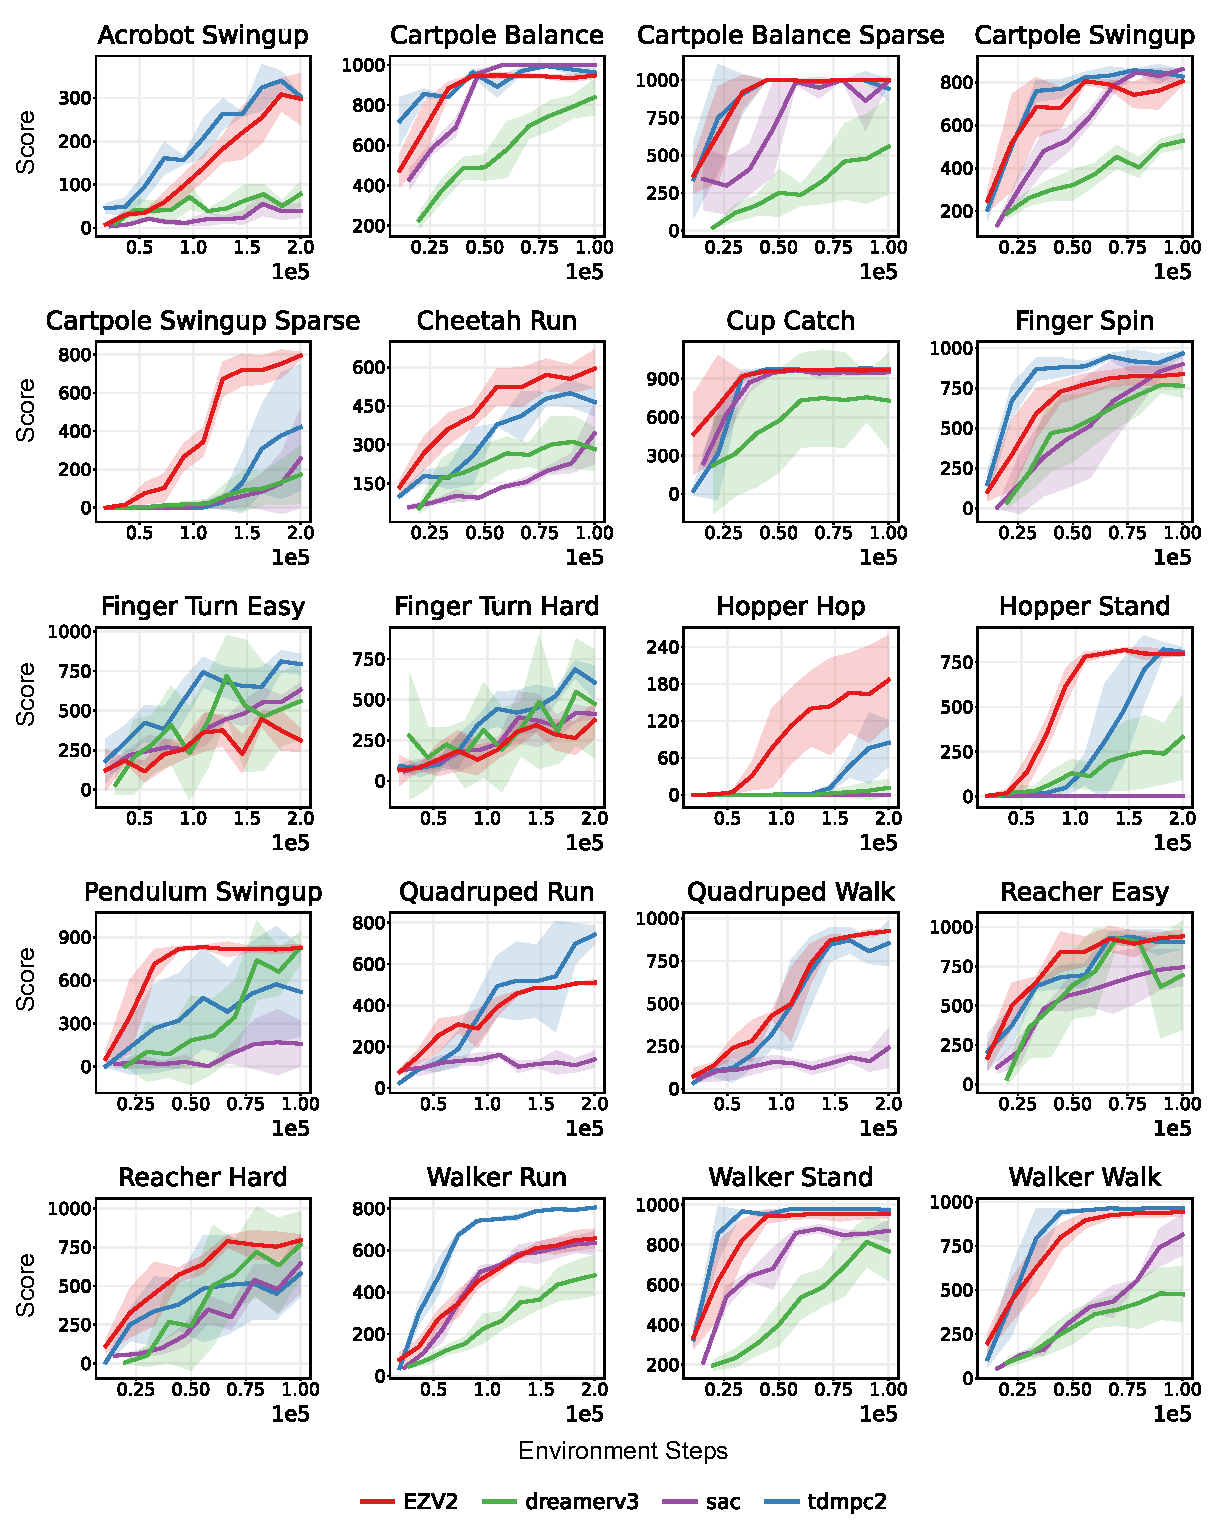
\includegraphics[width=0.9\textwidth]{sections/figs/dmc_proprio_app.pdf}
\caption{DMC scores for proprioceptive inputs with a budget of 200K frames. it corresponds to 100K steps due to the action repeat. (Because different algorithms have varying logging frequencies, the starting points are not the same.)}
\label{dmc_proprio}
\end{figure}


\begin{figure}[t]
\centering
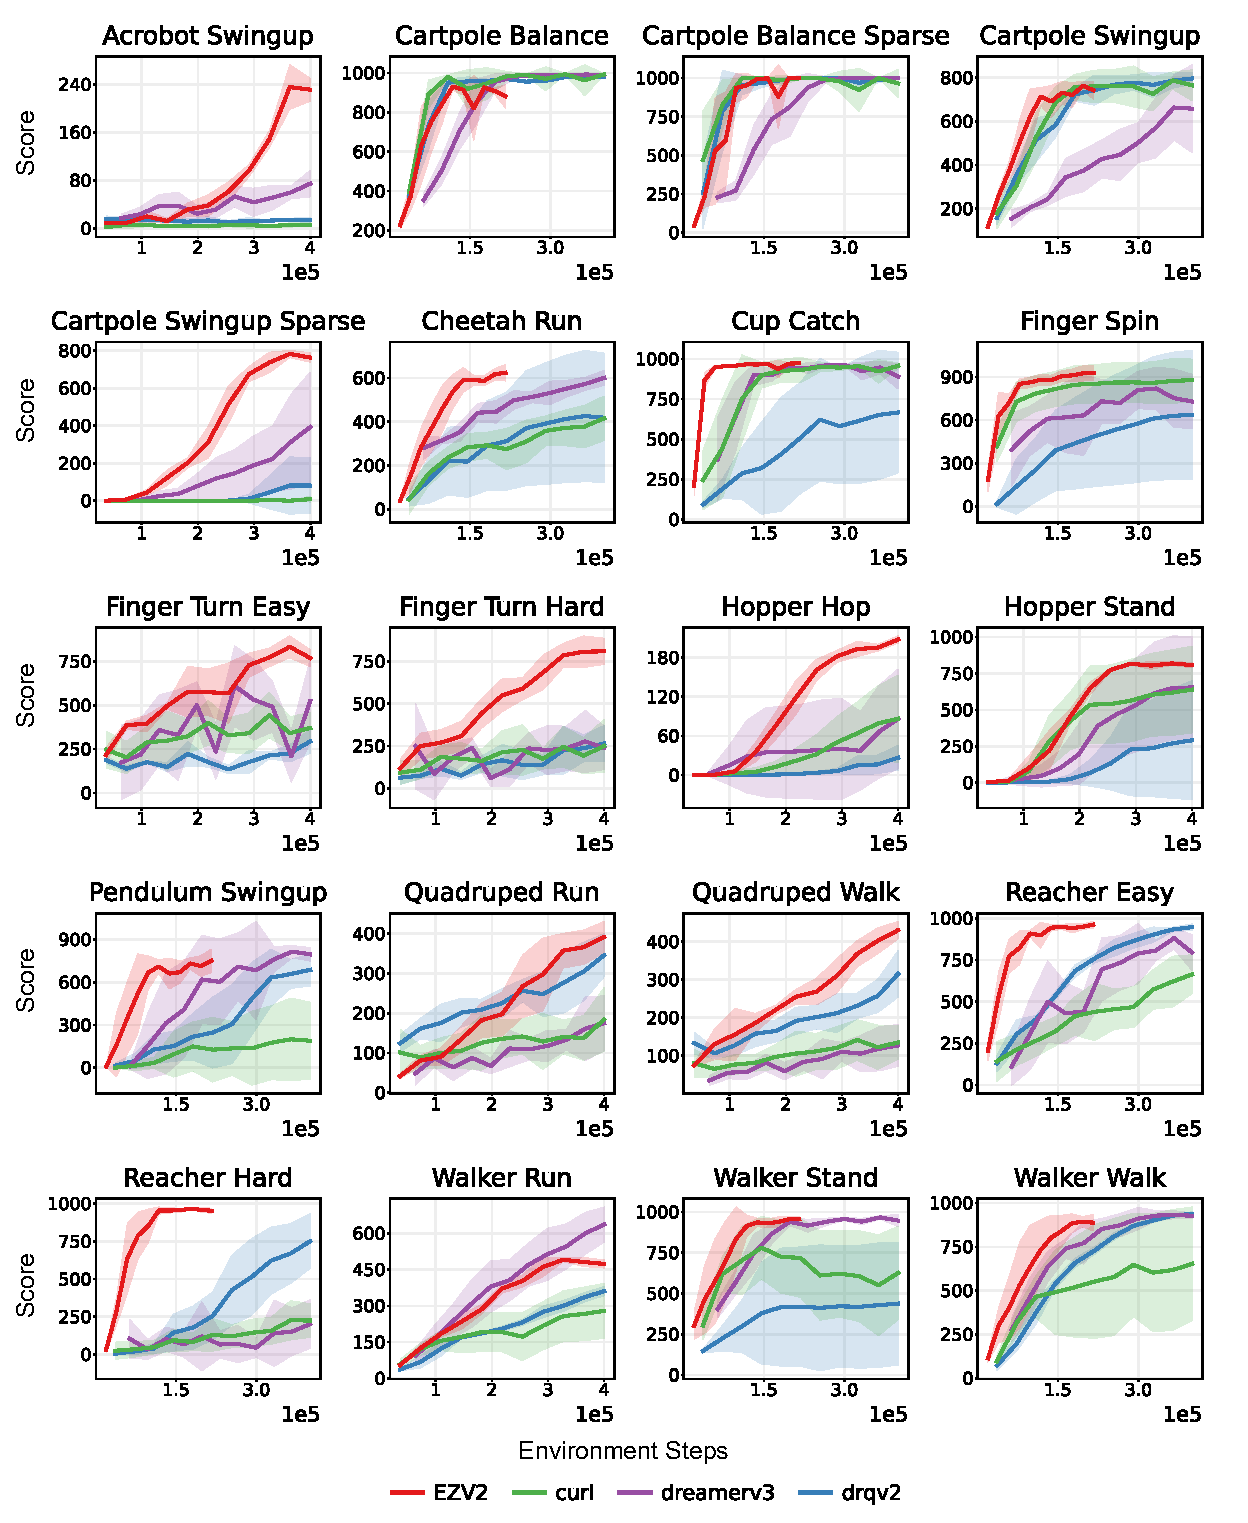
\includegraphics[width=0.9\textwidth]{sections/figs/dmc_vision_app.pdf}
\caption{DMC scores for image inputs with a budget of 400K frames. It corresponds to 200K steps due to the action repeat. (Because different algorithms have varying logging frequencies, the starting points are not the same.)}
\label{dmc_vision}
\end{figure}

\begin{figure}[t]
\centering
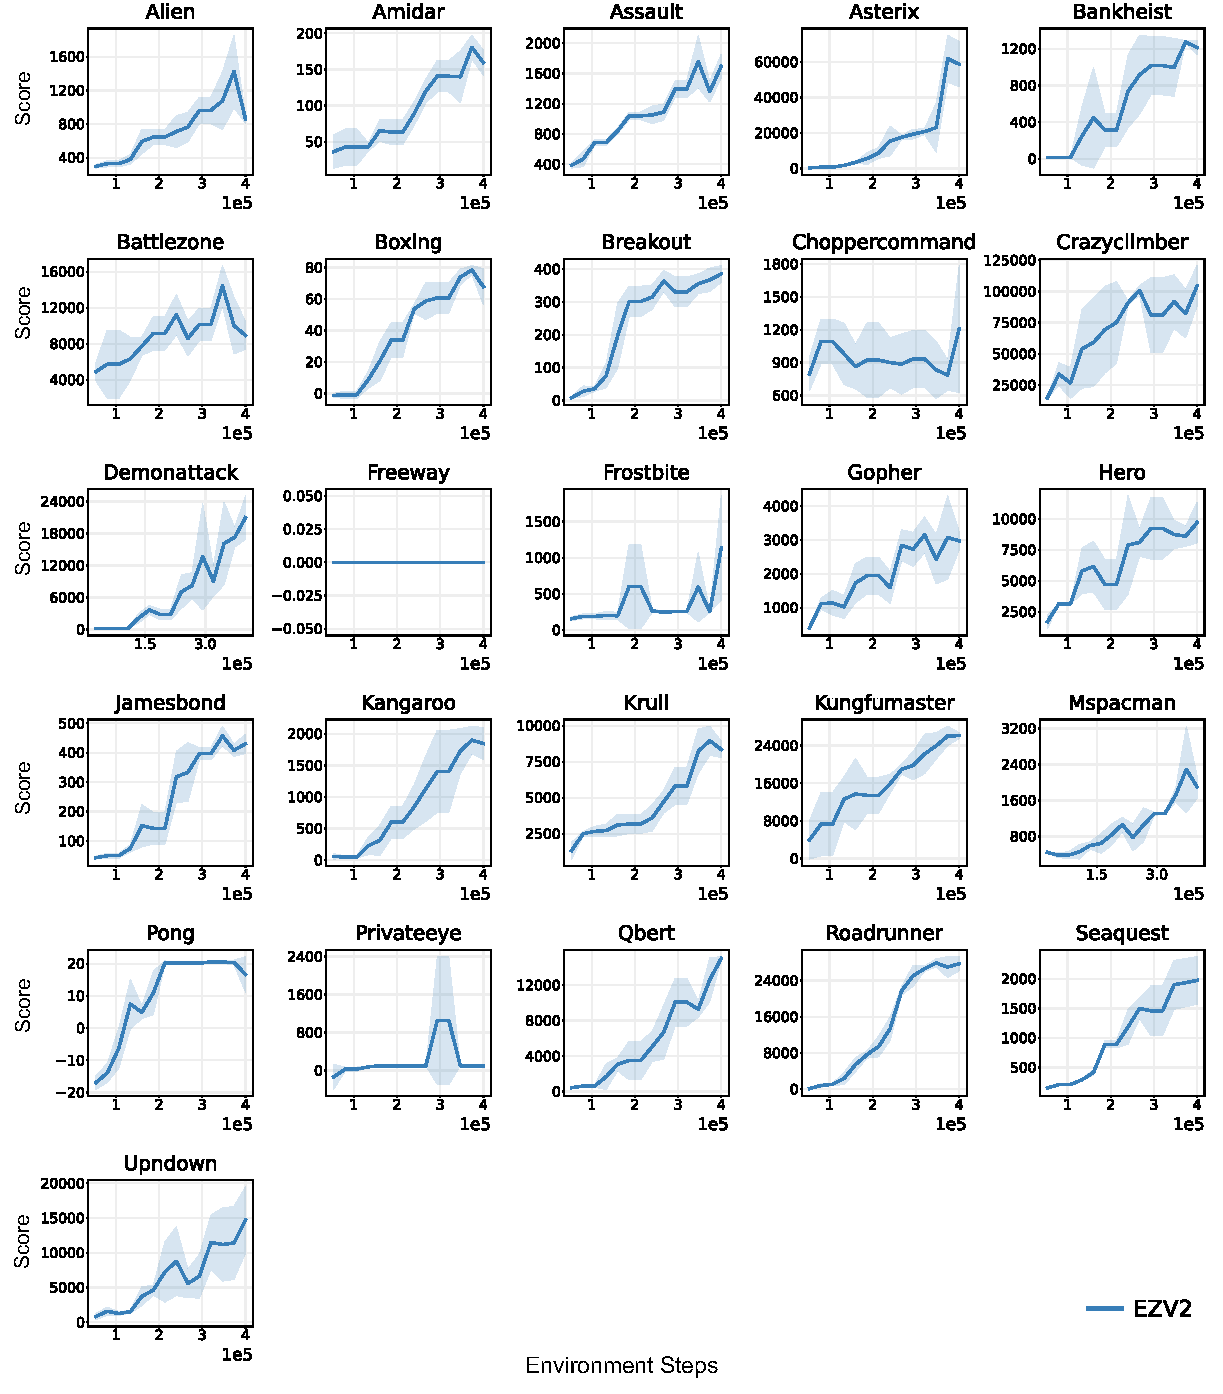
\includegraphics[width=0.9\textwidth]{sections/figs/atari_app.pdf}
\caption{Atari training curves with a budget of 400K frames, amounting to 100K interaction data.}
\label{atari}
\end{figure}

% \begin{figure}[t]
% \centering
% 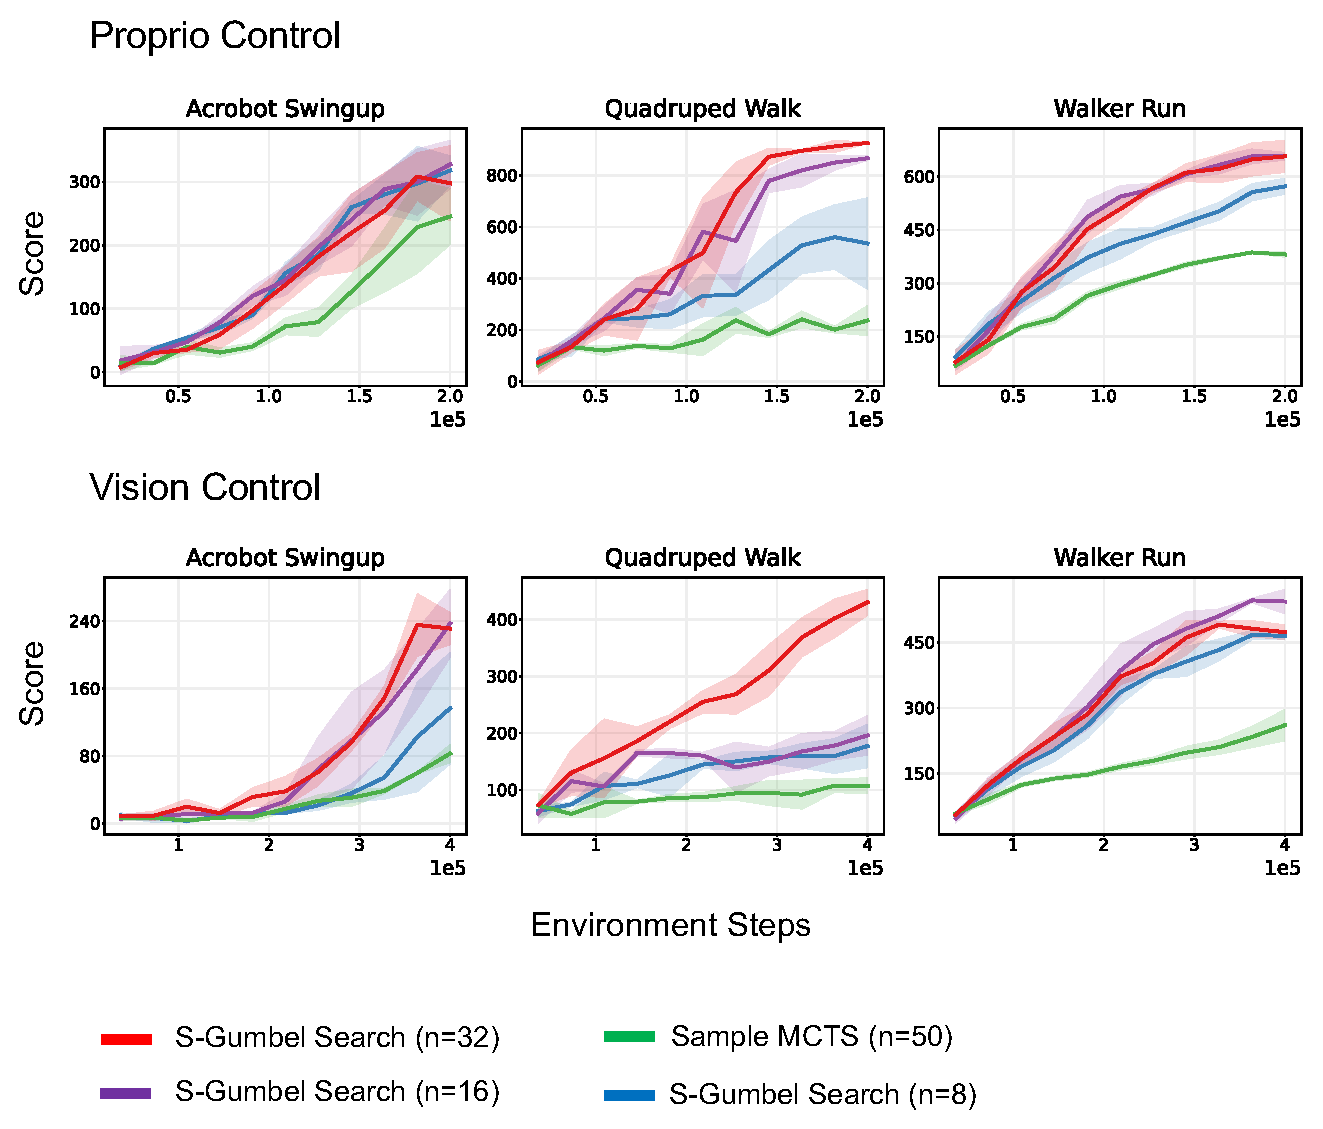
\includegraphics[width=0.75\textwidth]{sections/figs/ablation_search.pdf}
% \caption{The ablation study of our search method, namely sampling-based Gumbel search (S-Gumbel Search). Besides, we compare with sample MCTS \citep{hubert2021learning}, and our search method with different simulations.}
% \label{ablation_search}
% \end{figure}


% \begin{figure}[t]
% \centering
% 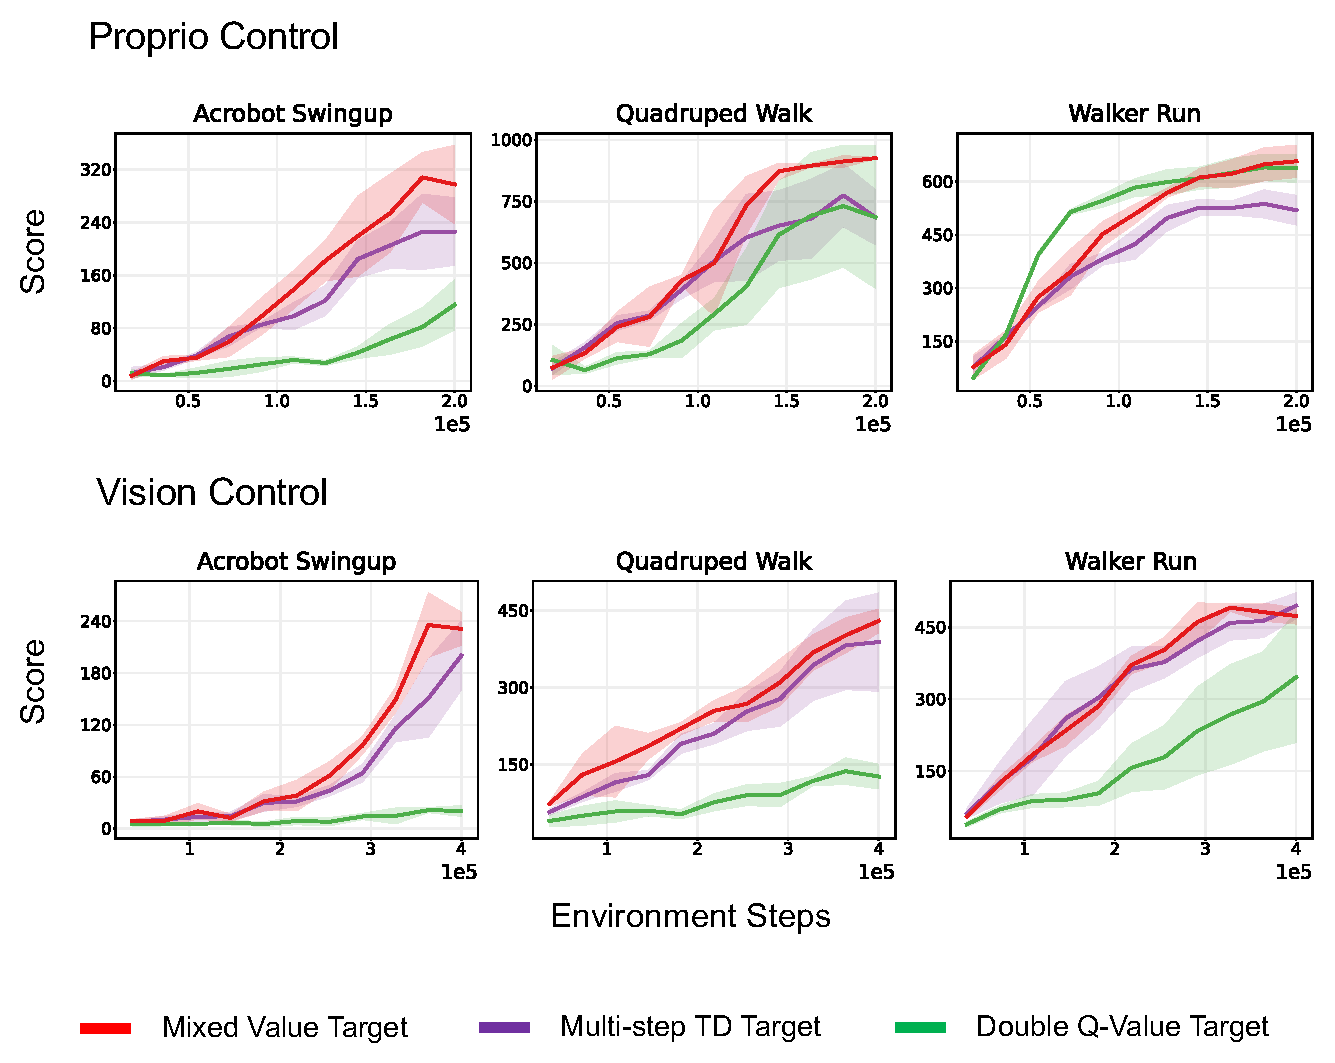
\includegraphics[width=0.75\textwidth]{sections/figs/ablation_value.pdf}
% \caption{The ablation study of the mixed value target we propose. Besides, we compare with multi-step TD target and double value target. Double Q-value target is similar to the value target in DDPG \cite{lillicrap2015continuous} (more details can be found in Section \ref{ablation_sec}).}
% \label{ablation_value}
% \end{figure}